% Options for packages loaded elsewhere
\PassOptionsToPackage{unicode}{hyperref}
\PassOptionsToPackage{hyphens}{url}
\PassOptionsToPackage{dvipsnames,svgnames,x11names}{xcolor}
%
\documentclass[
  11pt,
  letterpaper,
]{article}
\usepackage{amsmath,amssymb}
\usepackage{lmodern}
\usepackage{iftex}
\ifPDFTeX
  \usepackage[T1]{fontenc}
  \usepackage[utf8]{inputenc}
  \usepackage{textcomp} % provide euro and other symbols
\else % if luatex or xetex
  \usepackage{unicode-math}
  \defaultfontfeatures{Scale=MatchLowercase}
  \defaultfontfeatures[\rmfamily]{Ligatures=TeX,Scale=1}
\fi
% Use upquote if available, for straight quotes in verbatim environments
\IfFileExists{upquote.sty}{\usepackage{upquote}}{}
\IfFileExists{microtype.sty}{% use microtype if available
  \usepackage[]{microtype}
  \UseMicrotypeSet[protrusion]{basicmath} % disable protrusion for tt fonts
}{}
\makeatletter
\@ifundefined{KOMAClassName}{% if non-KOMA class
  \IfFileExists{parskip.sty}{%
    \usepackage{parskip}
  }{% else
    \setlength{\parindent}{0pt}
    \setlength{\parskip}{6pt plus 2pt minus 1pt}}
}{% if KOMA class
  \KOMAoptions{parskip=half}}
\makeatother
\usepackage{xcolor}
\IfFileExists{xurl.sty}{\usepackage{xurl}}{} % add URL line breaks if available
\IfFileExists{bookmark.sty}{\usepackage{bookmark}}{\usepackage{hyperref}}
\hypersetup{
  pdftitle={Quantifying the global burden of parental loss for children: a cause of death approach},
  colorlinks=true,
  linkcolor={blue},
  filecolor={Maroon},
  citecolor={blue},
  urlcolor={blue},
  pdfcreator={LaTeX via pandoc}}
\urlstyle{same} % disable monospaced font for URLs
\usepackage[margin=25mm]{geometry}
\usepackage{longtable,booktabs,array}
\usepackage{calc} % for calculating minipage widths
% Correct order of tables after \paragraph or \subparagraph
\usepackage{etoolbox}
\makeatletter
\patchcmd\longtable{\par}{\if@noskipsec\mbox{}\fi\par}{}{}
\makeatother
% Allow footnotes in longtable head/foot
\usepackage{footnote} % For some unknown reason, footnotehyper clashes with French
\makesavenoteenv{longtable}
\usepackage{graphicx}
\makeatletter
\def\maxwidth{\ifdim\Gin@nat@width>\linewidth\linewidth\else\Gin@nat@width\fi}
\def\maxheight{\ifdim\Gin@nat@height>\textheight\textheight\else\Gin@nat@height\fi}
\makeatother
% Scale images if necessary, so that they will not overflow the page
% margins by default, and it is still possible to overwrite the defaults
% using explicit options in \includegraphics[width, height, ...]{}
\setkeys{Gin}{width=\maxwidth,height=\maxheight,keepaspectratio}
% Set default figure placement to htbp
\makeatletter
\def\fps@figure{htbp}
\makeatother
\setlength{\emergencystretch}{3em} % prevent overfull lines
\providecommand{\tightlist}{%
  \setlength{\itemsep}{0pt}\setlength{\parskip}{0pt}}
\setcounter{secnumdepth}{5}
\newlength{\cslhangindent}
\setlength{\cslhangindent}{1.5em}
\newlength{\csllabelwidth}
\setlength{\csllabelwidth}{3em}
\newlength{\cslentryspacingunit} % times entry-spacing
\setlength{\cslentryspacingunit}{\parskip}
\newenvironment{CSLReferences}[2] % #1 hanging-ident, #2 entry spacing
 {% dont indent paragraphs
  \setlength{\parindent}{0pt}
  % turn on hanging indent if param 1 is 1
  \ifodd #1
  \let\oldpar\par
  \def\par{\hangindent=\cslhangindent\oldpar}
  \fi
  % set entry spacing
  \setlength{\parskip}{#2\cslentryspacingunit}
 }%
 {}
\usepackage{calc}
\newcommand{\CSLBlock}[1]{#1\hfill\break}
\newcommand{\CSLLeftMargin}[1]{\parbox[t]{\csllabelwidth}{#1}}
\newcommand{\CSLRightInline}[1]{\parbox[t]{\linewidth - \csllabelwidth}{#1}\break}
\newcommand{\CSLIndent}[1]{\hspace{\cslhangindent}#1}

%%%%%%%% START HEADER PARTIAL %%%%%%%%%%%%

% Formatting of tables & knitr::kable and kableExtra functionality
\usepackage{float}
\usepackage{colortbl}
\usepackage{pdflscape}
\usepackage{tabu}
\usepackage{threeparttable}

% Line numbering

% endfloat stuff

% fancyhdr pagestyle

% Environment for keywords
\makeatletter
\newcommand\keywordsname{Keywords}
\newenvironment*{keywords}[1][\keywordsname]{\if@twocolumn \else \small \quotation \fi \begin{center} \textbf{\textit{#1} \\}}{\end{center}\if@twocolumn \else \small \endquotation \fi}
\newenvironment*{keywordsinline}[1][\keywordsname]{\if@twocolumn \else \small \quotation \fi \begin{center} \textbf{\textit{#1}: }}{\end{center}\if@twocolumn \else \small \endquotation \fi}
\makeatother

% Environment for abstract that takes new abstract name
\newenvironment{renameableabstract}[1][\abstractname]{\let\oldabstractname\abstractname \renewcommand{\abstractname}{#1} \begin{abstract}}{\end{abstract} \renewcommand{\abstractname}{\oldabstractname}}

%%%%%%%% END HEADER PARTIAL %%%%%%%%%%%%

\ifLuaTeX
  \usepackage{selnolig}  % disable illegal ligatures
\fi

\title{Quantifying the global burden of parental loss for children: a cause of death approach}

%%%%%%% START AUTHOR PARTIAL %%%%%%%%%%%%%%%

%%%%% Authors, affiliations and author notes stuff %%%%%

% Macros for creating and referencing stored reference
\makeatletter
\def\MyNewLabel#1#2#3{\expandafter\gdef\csname #1@#2\endcsname{#3}}

\def\MyRef#1#2{\@ifundefined{#1@#2}{???}{\csname #1@#2\endcsname}}

\newcommand*\ifcounter[1]{%
  \ifcsname c@#1\endcsname
    \expandafter\@firstoftwo
  \else
    \expandafter\@secondoftwo
  \fi
}
\makeatother

% Create labels for Addresses if the are given by code
\MyNewLabel{ADDRTXT}{A}{Department of Statistical Sciences, University of Toronto, Canada}
\MyNewLabel{ADDRTXT}{B}{Leverhulme Centre for Demographic Science, University of Oxford, England}
\MyNewLabel{ADDRTXT}{C}{Kinship Inequalities Research Group, Max Planck Institute for Demographic Research, Germany}
\MyNewLabel{ADDRTXT}{D}{Departments of Statistical Sciences and Sociology, University of Toronto, Canada}

% Create labels for Footnotes if they are given by code
\MyNewLabel{ANOTETXT}{corresp}{\href{mailto:benjamin.schluter@utoronto.ca}{\nolinkurl{benjamin.schluter@utoronto.ca}}.}

%%% Special footnotes for addresses and author footnotes
\usepackage{bigfoot}
\DeclareNewFootnote{Addr}[arabic] % Only used for NOT authblk
\DeclareNewFootnote{ANote}[fnsymbol]

%%% Address and author notes as a function of format %%%
 % Use authblk for affiliations %%%%%%%%%%%
\usepackage{authblk}

% Always separate by commas
\renewcommand\Authsep{, }
\renewcommand\Authand{, }
\renewcommand\Authands{, }

% Counter for addresses and footnotes
\newcounter{addrcnt}

% thanks definition that doesnt produce superscript marks
\makeatletter
\newcommand*\createaddrlblbycode[1]{%
  \ifcounter{ADDRLBL@#1}
    {}
    {\refstepcounter{addrcnt}\newcounter{ADDRLBL@#1}\setcounter{ADDRLBL@#1}{\value{addrcnt}}}%
}

\newcommand*\addrlblbycode[1]{\arabic{ADDRLBL@#1}}

\newcommand*\addrbycode[1]{%
  \ifcounter{ADDR@#1}
    {}
    {\newcounter{ADDR@#1}%
     \affil[\addrlblbycode{#1}]{\MyRef{ADDRTXT}{#1}}}%
}

\newcommand*\createanotelblbycode[1]{%
  \ifcounter{ANOTELBL@#1}
    {}
    {\refstepcounter{footnoteANote}\newcounter{ANOTELBL@#1}\setcounter{ANOTELBL@#1}{\value{footnoteANote}}}%
}

\newcommand*\anotelblbycode[1]{\fnsymbol{ANOTELBL@#1}}

\newcommand*\anotebycode[1]{%
  \ifcounter{ANOTE@#1}
    {}
    {\newcounter{ANOTE@#1}%
     \footnotetextANote[\value{ANOTELBL@#1}]{\MyRef{ANOTETXT}{#1}}}%
}
\makeatother


\createaddrlblbycode{A}


\createanotelblbycode{corresp}

\author[%
\addrlblbycode{A}%
,%
$\anotelblbycode{corresp}$%
]{Benjamin-Samuel Schlüter}

\addrbycode{A}


\createaddrlblbycode{B}



\author[%
\addrlblbycode{B}%
]{Antonino Polizzi}

\addrbycode{B}


\createaddrlblbycode{C}



\author[%
\addrlblbycode{C}%
]{Diego Alburez-Gutierrez}

\addrbycode{C}


\createaddrlblbycode{D}



\author[%
\addrlblbycode{D}%
]{Monica Alexander}

\addrbycode{D}


%endif(authblk)

%%%%%%%%% END AUTHOR PARTIAL %%%%%%%%

\date{}

\begin{document}
\maketitle

%%%%%%%%%% START AFTER TITLE PARTIAL %%%%%%%%%%%%%
\anotebycode{corresp}


%%%%%%%%%% END AFTER TITLE PARTIAL %%%%%%%%%%%%%

\begin{abstract}
Parental loss has the potential to impair physical and mental well-being. The timing and cause of parental death are important mediators of the bereavement process. Previous research on the probability of parental loss has focused on a subset of causes of death in few countries. We aim to provide a global assessment of the role of different causes of death in the experience of orphanhood. Using estimates from the United Nations World Population Prospects and the Global Burden of Disease study, we apply a formal kinship matrix approach to estimate the probability and causes of parental loss worldwide. Although the probability of orphanhood has generally declined over time, children in the Global South are still more likely to experience bereavement. In countries such as Afghanistan, Mexico, and Zimbabwe, a large proportion of parental deaths are conflict- or epidemic-related. In the United States, the top cause of father bereavement is violent death.
\end{abstract}

\hypertarget{introduction}{%
\section{Introduction}\label{introduction}}

Shared lifetime between children and their parents is longer today than ever before. Declining fertility has led to shrinking kinship networks in many regions of the world during the 20th century. At the same time, widespread improvements in mortality conditions have increased the time shared between younger and older generations (\protect\hyperlink{ref-bengtson2001nuclear}{Bengtson 2001}), as, on average, children lose their parents later in life.

While mortality conditions have improved, the presence of premature adult death still means many children lose parents at a young age. Parental bereavement has the potential to impair physical and mental well-being (\protect\hyperlink{ref-amato2014death}{Amato and Anthony 2014}; \protect\hyperlink{ref-li2014mortality}{Li et al. 2014}; \protect\hyperlink{ref-luecken2008parental}{Luecken 2008}; \protect\hyperlink{ref-pham2018burden}{Pham et al. 2018}; \protect\hyperlink{ref-saarela2018mortality}{Saarela and Rostila 2019}), while the timing and cause of parental death are important mediators of the bereavement process (\protect\hyperlink{ref-li2014mortality}{Li et al. 2014}). The early and sudden loss of a parent has been shown to have a particularly negative impact on the well-being and development of affected children (\protect\hyperlink{ref-chen2009education}{Chen, Chen, and Liu 2009}; \protect\hyperlink{ref-leopold2015bereavement}{Leopold and Lechner 2015}; \protect\hyperlink{ref-patterson2020linked}{Patterson, Verdery, and Daw 2020}). In contrast, degenerative diseases, such as dementia and Alzheimer's disease, are associated with increased family caregiver burden before the parental death, with often detrimental effects on the caregivers' well-being and the quality of family relationships (\protect\hyperlink{ref-alzheimers2022}{Alzheimer's Association Report 2022}).

Despite the importance of assessing the causes of parental death to fully understand the bereavement process of children, our knowledge of the cause-of-death patterns in parental loss is limited. Previous research on parental loss has focused on a small number of countries to study the effects of Covid-19 (\protect\hyperlink{ref-hillis2021global}{Susan D. Hillis et al. 2021b}; \protect\hyperlink{ref-hillis2021us}{Susan D. Hillis et al. 2021a}; \protect\hyperlink{ref-snyder2022covid}{Snyder et al. 2022}; \protect\hyperlink{ref-verdery2020covid}{Verdery et al. 2020}) and the HIV/AIDS epidemic (\protect\hyperlink{ref-zagheni2011impact}{Zagheni 2011}).

Kin loss is not just the product of present mortality rates. The probability of losing a parent is affected by the fertility rates of the parental generation (which determine the number of children `at risk' of orphanhood), the past mortality conditions affecting the parental and child generation (i.e., if both parents have already died, a child is no longer at risk of orphanhood), and the present mortality conditions (which determine the risk that a parent will die in a given year). Consequently, as countries differ in their mortality and fertility conditions as well as their epidemiological profiles (\protect\hyperlink{ref-owid-causes-of-death}{Dattani et al. 2023}; \protect\hyperlink{ref-united2022world}{United Nations 2022}), the short- and long-term burden associated with parental loss can be expected to vary across the globe.

In this project, we aim to provide a global assessment of the role of different causes of death in the experience of parental loss. We use a formal kinship matrix approach (\protect\hyperlink{ref-caswell2019formal}{Caswell 2019}) in combination with mortality and fertility data from the United Nations World Population Prospects (UNWPP), and cause-of-death information from the Global Burden of Disease (GBD) study to estimate causes of parental bereavement. In this extended abstract, we present preliminary results for four countries: Afghanistan, Mexico, United States of America (USA), and Zimbabwe.

\hypertarget{data-and-methods}{%
\section{Data and Methods}\label{data-and-methods}}

We combined two sources of data to estimate the worldwide parental loss by cause of death: cause-specific mortality, and life table data with its associated population counts, and fertility rates.

We used the 2022 Revision of World Population Prospects (\protect\hyperlink{ref-united2022world}{United Nations 2022}) to obtain period life tables by sex; period fertility rates for females aged 15 to 49 years old, and yearly population counts by sex, all by 1-year age class and grouped into individual calendar years over the period 1950--2019. Cause of death information was obtained from modeled data from the Global Burden of Disease (GBD) study (\protect\hyperlink{ref-ihme2019gbd}{Institute for Health Metrics and Evaluation 2019}) available over the period 1990--2019. Cause of death information was collected from this source for ages 0, 1--4, and then in five-year age groups until the open age group 95 and more. We converted these counts into 1-year age groups until age 100+, using a penalized composite link model (\protect\hyperlink{ref-rizzi2015efficient}{Rizzi, Gampe, and Eilers 2015}). Twenty-two causes of death were selected corresponding to level two of the GBD hierarchy of causes.

In order to estimate parental loss by cause, we used the kinship matrix projection model developed by Caswell (\protect\hyperlink{ref-caswell2019formal}{2019}) focusing only on the projected kin that are parent (mother and father). The model combined several extensions to use time-varying and sex-differentiated vital rates while accounting for death from multiple causes (\protect\hyperlink{ref-caswell2022formal}{Caswell 2022}; \protect\hyperlink{ref-caswell2023formal}{Caswell, Margolis, and Verdery 2023}; \protect\hyperlink{ref-caswell2021formal}{Caswell and Song 2021}). The projection model for parents can be expressed as follows:

\[\begin{pmatrix} \boldsymbol{d}^f_L \\ 
\boldsymbol{d}^m_L \\ 
\hline \boldsymbol{d}^f_D \\ 
\boldsymbol{d}^m_D 
\end{pmatrix}(x+1, t+1) = 
\left(\begin{array}{@{}c|c@{}}
  \begin{matrix} 
  \boldsymbol{U}^f_t & \boldsymbol{0} \\ 
  \boldsymbol{0} & \boldsymbol{U}^m_t 
  \end{matrix} & \boldsymbol{0} \\
\hline
\begin{matrix} 
  \boldsymbol{M}^f_t & \boldsymbol{0} \\ 
  \boldsymbol{0} & \boldsymbol{M}^m_t 
  \end{matrix} & \boldsymbol{0} \\
\end{array}\right)
\begin{pmatrix} \boldsymbol{d}^f_L \\ 
\boldsymbol{d}^m_L \\ 
\hline \boldsymbol{d}^f_D \\ 
\boldsymbol{d}^m_D
\end{pmatrix}(x, t)\]

where \(\omega=101\) is the number of ages considered; \(\alpha=22\) are the twenty-two different causes of death considered; the matrix \(\boldsymbol{U}_t\) of dimension \((\omega \times \omega)\) contains the survival probabilities on its main subdiagonal; the matrix \(\boldsymbol{M}_t\) of dimension \((\alpha\omega \times \omega)\) contains the probabilities of dying from the causes considered on its main diagonals; \(\boldsymbol{d}_L\) refers to the age distribution of the parent living and \(\boldsymbol{d}_D\) reflects the age distribution of the parent dying by cause, in year \(t\) when a child is aged \(x\); upper scripts \(f\) and \(m\) correspond to female and male, respectively; subscript \(t\) refers to the year. The block matrix on the right-hand side allows to project the parents' age distribution (alive or dead) over time, as their child ages. The model is fit to each country separately.\\
The model requires as input the age distribution of parents of offspring (see Caswell and Song (\protect\hyperlink{ref-caswell2021formal}{2021}) for more details). We assumed that in a given year \(t\), both parents were alive at the time of birth and the age distribution of parents at the birth of their child (when \(x=0\)) is expressed as \(\boldsymbol{\pi_t} = \frac{\boldsymbol{f}_t \circ \boldsymbol{n}_t}{||\boldsymbol{f}_t \circ \boldsymbol{n}_t||}\), where \(\boldsymbol{f}_t\) is a vector of dimension \((\omega \times 1)\) containing age-specific fertility rates and \(\boldsymbol{n}_t\) is a vector of dimension \((\omega \times 1)\) being the age distribution of the overall population. Hence, at the birth of a child in year \(t\),

\[\begin{pmatrix} \boldsymbol{d}^f_L \\ 
\boldsymbol{d}^m_L \\ 
\hline \boldsymbol{d}^f_D \\ 
\boldsymbol{d}^m_D 
\end{pmatrix}(0, t)
=
\begin{pmatrix} \boldsymbol{\pi_t}^f \\ 
\boldsymbol{\pi_t}^m \\ 
\hline \boldsymbol{0} \\ 
\boldsymbol{0} 
\end{pmatrix}
\]

We assumed that female and male age-specific fertility rates were equal as the UN does not provide data on male fertility (\protect\hyperlink{ref-alburez2023projections}{Alburez-Gutierrez, Williams, and Caswell 2023}).
Cause-specific mortality was not available for the period 1950--1990. During this period, we simplified the block-matrix to only contain survival probabilities, meaning that we only projected the age distribution of parents alive before 1990 (\(\boldsymbol{M}_t = \boldsymbol{0}\) for \(t < 1990\)). We additionally recorded the age distribution of parents dying by cause from 1990 until 2019. As it is commonly done in these models (\protect\hyperlink{ref-snyder2022covid}{Snyder et al. 2022}; \protect\hyperlink{ref-verdery2020covid}{Verdery et al. 2020}), before 1950, we assumed that the earliest available rates operated for a long time (stable population assumption).

The kinship matrix projection model provides the mean numbers of parental deaths (\(d_D(x)\)) for a child at every age \(x\). The sum of the mean numbers of parental deaths over the child's life course is equal to two as we consider mother and father. In order to convert the mean number of parental deaths into the probability that a child experiences such a death at a given age, we assumed that the number of parental deaths at age \(x\) is binomially distributed (similarly to Caswell, Margolis, and Verdery (\protect\hyperlink{ref-caswell2023formal}{2023})),

\[\text{Pr.(losing k parents)}_x = \binom{2}{k}\left(\frac{d_D(x)}{2}\right)^k\left(1-\frac{d_D(x)}{2}\right)^{2-k}.\]

Hence, the probability of losing at least one parent at age \(x\) is computed as follows,

\[\text{Pr.(losing at least one parent)}_x = 1 - \text{Pr.(losing 0 parent)}_x = 1 -  \left(1-\frac{d_D(x)}{2}\right)^2.\]
Finally, obtaining the probability of children under 18 losing at least one parent can be expressed as follows,

\[\text{Pr.(losing at least one parent)}_{<18} = 1 - \left(1-\frac{\sum^{17}_{x=0}d_D(x)}{2}\right)^2.\]

\hypertarget{preliminary-results}{%
\section{Preliminary Results}\label{preliminary-results}}

Figure 1 shows the proportion of children under 18 years old who ever lost a father (left panel) or mother (right panel) over the period 1970--2019 for the four selected countries, Afghanistan, Mexico, the United States, and Zimbabwe. There are clear differences in country-specific trends over time. In the U.S., the probability of paternal orphanhood remained relatively constant over the five decades of observation, at about 5\%, while this probability declined sharply between the 1970s and the mid-2000s in Mexico. In Afghanistan, the probability of paternal death also showed a declining trend, with the exception of the periods 1979--1992 and 2017--2019, which were marked by large-scale conflict. Zimbabwe represents an exception to the general trend of low or declining paternal bereavement, with the likelihood of ever having lost a father increasing sharply during the 1980s and 1990s, which coincided with the HIV/AIDS crisis. During the 2010s, the likelihood of paternal bereavement in Zimbabwe started to decline again.

While the probability of maternal orphanhood was generally lower than the one of paternal orphanhood, trends in maternal and paternal bereavement followed similar trends in each country. Probabilities of maternal bereavement were usually affected little by periods of conflict (e.g., Afghanistan in the 1980s, 1977--1979 in Zimbabwe).

\begin{figure}
\centering
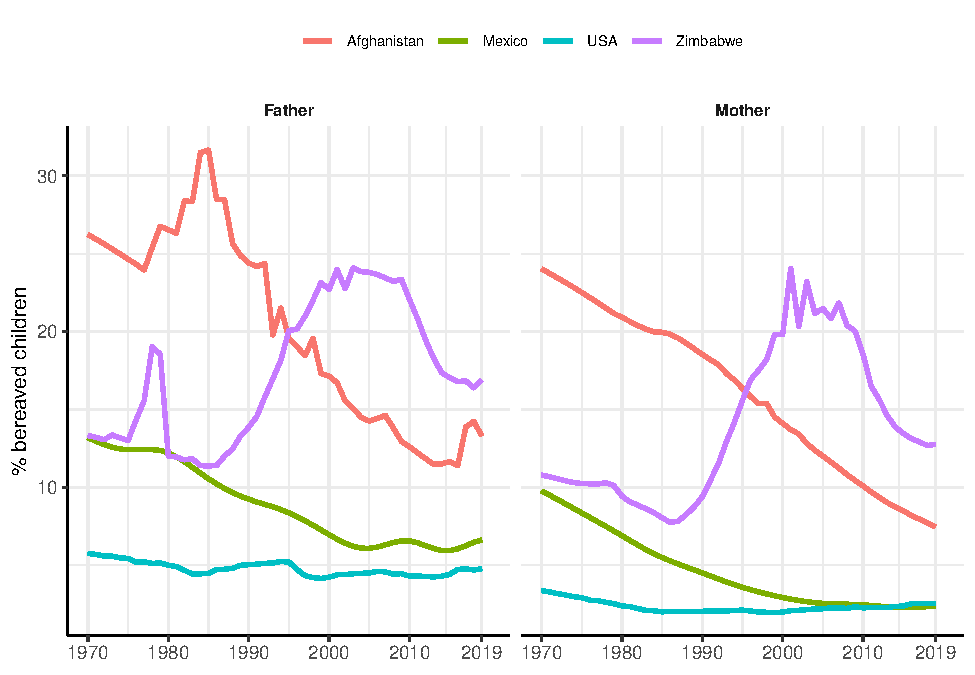
\includegraphics{parental_loss_global_paa_ext_abstract_files/figure-latex/perc-ber-all-1.pdf}
\caption{\label{fig:perc-ber-all}Percent of children that ever lost a parent, by parent sex and country over period 1970-2019}
\end{figure}

Figure 2 breaks down the proportion of paternal and maternal bereavement among children under 18 years old by causes of death for the period 1990--2019. For each country-sex combination, the proportion of paternal and maternal orphanhood is shown for the top three causes of death over the entire thirty-year period.

In line with trends displayed in Figure 1, paternal and maternal bereavement from ``self-harm and interpersonal violence'', ``cardiovascular diseases'', and ``neoplasms'' in the United States have displayed relatively stagnant trends in the 21st century. Similarly, following the all-cause trends in Figure 1, maternal bereavement from ``cardiovascular diseases'', ``maternal and neonatal disorders'', and ``neoplasms'' in Afghanistan and maternal bereavement from ``neoplasms'', ``cardiovascular diseases'', and ``diabetes and kidney diseases'' in Mexico showed declining trends, albeit to varying degrees. In Zimbabwe, parental bereavement due to ``HIV/AIDS and sexually transmitted infections'' clearly stands out as the driver of the all-cause trends shown in Figure 1. At the peak of the HIV/AIDS crisis in Zimbabwe, 16\% of children had previously lost their father to ``HIV/AIDS and sexually transmitted infections'', while 20\% of children had previously lost their mother. Finally, offsetting trends among different causes of death were seen for fathers in Afghanistan and Mexico, where, at different time points, high and rising bereavement from ``self-harm and interpersonal violence'' counteracted improvements in the remaining two causes of death (Afghanistan: ``cardiovascular diseases'' and ``transport injuries''; Mexico: ``digestive diseases'' and ``transport injuries'').

\begin{figure}
\centering
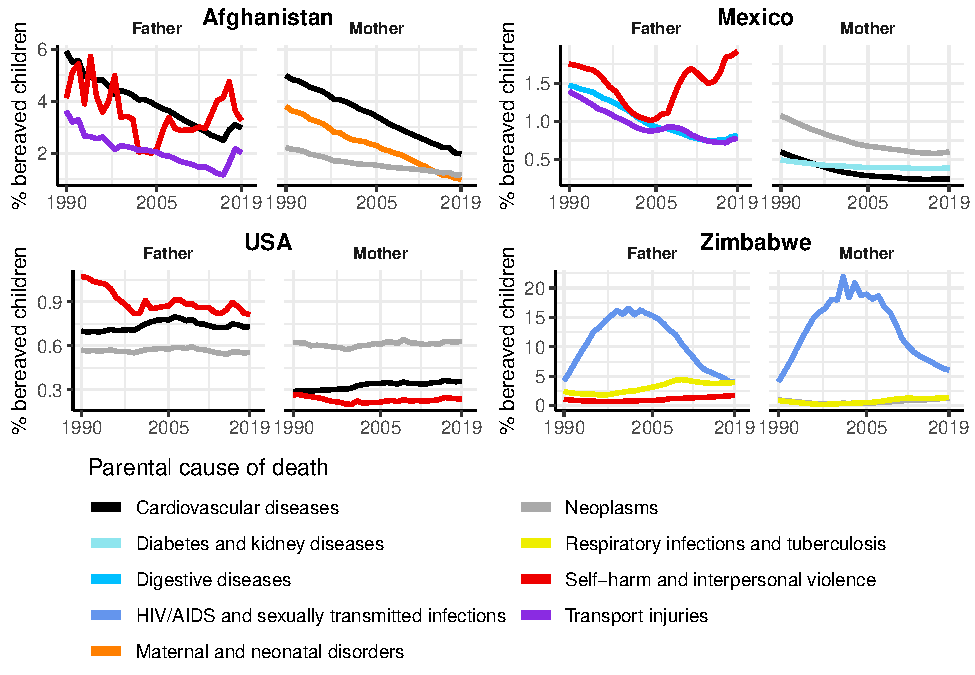
\includegraphics{parental_loss_global_paa_ext_abstract_files/figure-latex/perc-ber-top-1.pdf}
\caption{\label{fig:perc-ber-top}Percent of children that ever lost a parent, by parent sex and country top three causes of parental death over period 1990-2019}
\end{figure}

Finally, focusing on the age distribution of parental loss, Figure 3 shows the probability (y-axis) of losing at least one parent (father or mother) by age (x-axis) and cause of death (area color) in Afghanistan (left) and Mexico (right) in the year 2019. The top panels show the probability of parental loss from ``cardiovascular diseases'' and ``neoplasms'', while the bottom panels focus on the remaining top ten causes of death in each country in 2019 (excluding ``cardiovascular diseases'' and ``neoplasms'').

In line with Figure 1, the probability of having lost a parent was higher in childhood (i.e., areas for top twelve causes below age 18) in Afghanistan than in Mexico. Looking at the bottom panel of Figure 3, it becomes clear that ``self-harm and interpersonal violence'', ``transport injuries'', and ``unintentional injuries'' were the main contributors to this pattern.

The adult peak of parental loss was reached at around age 50 in Afghanistan and at around age 60 in Mexico. Parental loss from ``self-harm and interpersonal violence'' was more important for parental loss at all ages in Afghanistan. In contrast, ``diabetes and kidney diseases'', ``digestive diseases'', and ``neurological disorders'' played a more important role in Mexico.

\begin{figure}
\centering
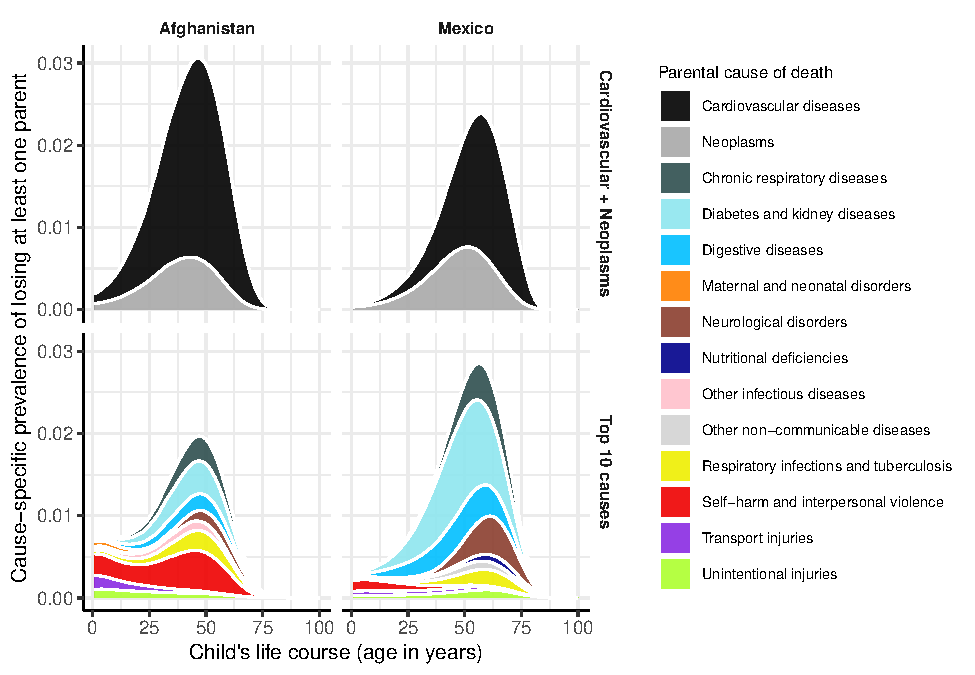
\includegraphics{parental_loss_global_paa_ext_abstract_files/figure-latex/ber-prob-1.pdf}
\caption{\label{fig:ber-prob}Age- and cause-specific probabilities of losing at least one parent, by country top twelve causes in 2019}
\end{figure}

\hypertarget{summary-discussion-and-next-steps}{%
\section{Summary, Discussion, and Next Steps}\label{summary-discussion-and-next-steps}}

In our project, we aim to provide a global assessment of the role of different causes of death in the experience of parental loss. Using a formal matrix approach, our study highlights the stark global differences in the experience of parental loss. Although the probability of orphanhood has generally declined over time, children in the Global South are still more likely to lose a parent. In the second half of the 20th century, many countries in the Global South, such as Afghanistan, Mexico, and Zimbabwe, have experienced short- or longer-term mortality crises resulting from conflicts or epidemics. These mortality crises have temporarily exacerbated experiences of parental loss (as in Afghanistan and Zimbabwe) or slowed down improvements in parental longevity (as in Mexico). Our findings show that in countries such as Afghanistan, Mexico, and Zimbabwe, a large proportion of parental deaths are conflict- or epidemic-related and can occur suddenly in a context already marked by social upheaval. Moreover, in Afghanistan, the high probability of mortality from maternal and neonatal disorders suggests that many children may grow up without a mother. While parental loss is less common in the United States, a large proportion of bereaved children in the U.S. have lost their father to a violent death. Future work will focus on presenting and interpreting results for all countries and deriving region-based estimates.

The preliminary results presented in this extended abstract represent only a small subset of countries and are subject to two main limitations. First, in many data-scarce contexts, the age-specific mortality and fertility rates and the cause-of-death information provided by UNWPP and GBD represent estimated quantities themselves. Consequently, biases in the mortality and fertility information are carried over to the estimates of parental loss derived from our matrix kinship models. GBD, and in some instances UNWPP, provide uncertainty bounds around their mortality and fertility estimates. For the PAA 2024 annual meeting, we aim to explicitly incorporate this uncertainty in our estimates of parental loss. Moreover, for selected countries, such as the United States and Mexico, we plan to conduct robustness checks with cause-of-death information derived directly from vital registration systems.

Second, in the absence of male fertility data, we approximate male fertility rates using an ``androgynous model'' to derive kin estimates, which assumes that female and male fertility patterns in a given country are identical. Existing information on female and male fertility suggests that the reproductive period of males is generally longer and the mean age of childbirth higher (\protect\hyperlink{ref-dudel2021fertility}{Dudel and Klüsener 2021}; \protect\hyperlink{ref-Schoumaker2019}{Schoumaker 2019}). Estimates of kin relationships derived from population registers vs.~matrix models for Sweden suggest that the ``androgynous model'' approximates register-based estimates of different kin relationships reasonably well (\protect\hyperlink{ref-alburez2023projections}{Alburez-Gutierrez, Williams, and Caswell 2023}). For the PAA 2024 annual meeting, we aim to test the sensitivity of our results to different assumptions about male fertility patterns.

Despite these limitations, our study provides important insights into the cause-of-death patterns in parental loss in different world regions. Against general increases in shared lifetime between children and their parents, our results suggest important variations in the short- and long-term burdens associated with parental loss across the globe. Thus, our findings will prove useful in the design of adequate support systems that help underage and adult children in their grieving process and protect children from potential social and economic repercussions arising from the death of their parents.

\newpage

\hypertarget{references}{%
\section*{References}\label{references}}
\addcontentsline{toc}{section}{References}

\hypertarget{refs}{}
\begin{CSLReferences}{1}{0}
\leavevmode\vadjust pre{\hypertarget{ref-alburez2023projections}{}}%
Alburez-Gutierrez, D., Williams, I., and Caswell, H. (2023). Projections of human kinship for all countries. doi:\href{https://doi.org/10.31235/osf.io/hn3zm}{10.31235/osf.io/hn3zm}.

\leavevmode\vadjust pre{\hypertarget{ref-alzheimers2022}{}}%
Alzheimer's Association Report (2022). 2022 {A}lzheimer's disease facts and figures. \emph{{A}lzheimer's \& Dementia} 18(4):700--789. doi:\href{https://doi.org/10.1002/alz.12638}{10.1002/alz.12638}.

\leavevmode\vadjust pre{\hypertarget{ref-amato2014death}{}}%
Amato, P.R. and Anthony, C.J. (2014). Estimating the effects of parental divorce and death with fixed effects models. \emph{Journal of Marriage and Family} 76(2):370--386. doi:\href{https://doi.org/10.1111/jomf.12100}{10.1111/jomf.12100}.

\leavevmode\vadjust pre{\hypertarget{ref-bengtson2001nuclear}{}}%
Bengtson, V.L. (2001). Beyond the nuclear family: The increasing importance of multigenerational bonds. \emph{Journal of Marriage and Family} 63(1):1--16. doi:\href{https://doi.org/10.1111/j.1741-3737.2001.00001.x}{10.1111/j.1741-3737.2001.00001.x}.

\leavevmode\vadjust pre{\hypertarget{ref-caswell2019formal}{}}%
Caswell, H. (2019). The formal demography of kinship. \emph{Demographic Research} 41:679--712.

\leavevmode\vadjust pre{\hypertarget{ref-caswell2022formal}{}}%
Caswell, H. (2022). The formal demography of kinship IV. \emph{Demographic Research} 47:359--396.

\leavevmode\vadjust pre{\hypertarget{ref-caswell2023formal}{}}%
Caswell, H., Margolis, R., and Verdery, A.M. (2023). The formal demography of kinship v: Kin loss, bereavement, and causes of death. \emph{SocArXiv}. doi:\href{https://doi.org/10.31235/osf.io/mk64p}{10.31235/osf.io/mk64p}.

\leavevmode\vadjust pre{\hypertarget{ref-caswell2021formal}{}}%
Caswell, H. and Song, X. (2021). The formal demography of kinship III. \emph{Demographic Research} 45:517--546.

\leavevmode\vadjust pre{\hypertarget{ref-chen2009education}{}}%
Chen, S.H., Chen, Y.-C., and Liu, J.-T. (2009). The impact of unexpected maternal death on education: First evidence from three national administrative data links. \emph{The American Economic Review} 99(2):149--153. doi:\href{https://doi.org/10.1257/aer.99.2.149}{10.1257/aer.99.2.149}.

\leavevmode\vadjust pre{\hypertarget{ref-owid-causes-of-death}{}}%
Dattani, S., Spooner, F., Ritchie, H., and Roser, M. (2023). \emph{Causes of Death}. Our World in Data. \url{https://ourworldindata.org/causes-of-death}.

\leavevmode\vadjust pre{\hypertarget{ref-dudel2021fertility}{}}%
Dudel, C. and Klüsener, S. (2021). Male--female fertility differentials across 17 high-income countries: Insights from a new data resource. \emph{European Journal of Population} 37(2):417--441. doi:\href{https://doi.org/10.1007/s10680-020-09575-9}{10.1007/s10680-020-09575-9}.

\leavevmode\vadjust pre{\hypertarget{ref-hillis2021us}{}}%
Hillis, Susan D., Blenkinsop, A., Villaveces, A., Annor, F.B., Liburd, L., Massetti, G.M., Demissie, Z., Mercy, J.A., Nelson III, C.A., Cluver, L., Flaxman, S., Sherr, L., Donnelly, C.A., Ratmann, O., and Unwin, H.J.T. (2021a). COVID-19-associated orphanhood and caregiver death in the {U}nited {S}tates. \emph{Pediatrics} 148(6):e2021053760. doi:\href{https://doi.org/10.1542/peds.2021-053760}{10.1542/peds.2021-053760}.

\leavevmode\vadjust pre{\hypertarget{ref-hillis2021global}{}}%
Hillis, Susan D., Unwin, H.J.T., Chen, Y., Cluver, L., Sherr, L., Goldman, P.S., Ratmann, O., Donnelly, C.A., Bhatt, S., Villaveces, A., Butchart, A., Bachman, G., Rawlings, L., Green, P., Nelson III, C.A., and Flaxman, S. (2021b). Global minimum estimates of children affected by COVID-19-associated orphanhood and deaths of caregivers: A modelling study. \emph{The Lancet} 398(10298):391--402. doi:\href{https://doi.org/10.1016/S0140-6736(21)01253-8}{10.1016/S0140-6736(21)01253-8}.

\leavevmode\vadjust pre{\hypertarget{ref-ihme2019gbd}{}}%
Institute for Health Metrics and Evaluation (2019). \emph{GBD Results}. University of Washington. \url{https://vizhub.healthdata.org/gbd-results/}.

\leavevmode\vadjust pre{\hypertarget{ref-leopold2015bereavement}{}}%
Leopold, T. and Lechner, C.M. (2015). Parents' death and adult well-being: Gender, age, and adaptation to filial bereavement. \emph{Journal of Marriage and Family} 77(3):747--760. doi:\href{https://doi.org/10.1111/jomf.12186}{10.1111/jomf.12186}.

\leavevmode\vadjust pre{\hypertarget{ref-li2014mortality}{}}%
Li, J., Vestergaard, M., Cnattingius, S., Gissler, M., Bech, B.H., Obel, C., and Olsen, J. (2014). Mortality after parental death in childhood: A nationwide cohort study from three nordic countries. \emph{PLOS Medicine} 11(7):e1001679. doi:\href{https://doi.org/10.1371/journal.pmed.1001679}{10.1371/journal.pmed.1001679}.

\leavevmode\vadjust pre{\hypertarget{ref-luecken2008parental}{}}%
Luecken, L.J. (2008). Long-term consequences of parental death in childhood: Psychological and physiological manifestations. In: Stroebe, M. S., Hansson, R. O., Schut, H. and Stroebe, W. (eds.). \emph{Handbook of Bereavement Research and Practice: Advances in Theory and Intervention}. Washington, D.C.: American Psychological Association: 397--416. doi:\href{https://doi.org/10.1037/14498-019}{10.1037/14498-019}.

\leavevmode\vadjust pre{\hypertarget{ref-patterson2020linked}{}}%
Patterson, S.E., Verdery, A.M., and Daw, J. (2020). Linked lives and childhood experience of family death on educational attainment. \emph{Socius} 6:2378023120975594.

\leavevmode\vadjust pre{\hypertarget{ref-pham2018burden}{}}%
Pham, S., Porta, G., Biernesser, C., Walker Payne, M., Iyengar, S., Melhem, N., and Brent, D.A. (2018). The burden of bereavement: Early-onset depression and impairment in youths bereaved by sudden parental death in a 7-year prospective study. \emph{American Journal of Psychiatry} 175(9):887--896.

\leavevmode\vadjust pre{\hypertarget{ref-rizzi2015efficient}{}}%
Rizzi, S., Gampe, J., and Eilers, P.H. (2015). Efficient estimation of smooth distributions from coarsely grouped data. \emph{American Journal of Epidemiology} 182(2):138--147.

\leavevmode\vadjust pre{\hypertarget{ref-saarela2018mortality}{}}%
Saarela, J. and Rostila, M. (2019). Mortality after the death of a parent in adulthood: A register-based comparison of two ethno-linguistic groups. \emph{European Journal of Public Health} 29(3):582--587. doi:\href{https://doi.org/10.1093/eurpub/cky189}{10.1093/eurpub/cky189}.

\leavevmode\vadjust pre{\hypertarget{ref-Schoumaker2019}{}}%
Schoumaker, B. (2019). Male fertility around the world and over time: How different is it from female fertility? \emph{Population and Development Review} 45:459--487. \url{https://about.jstor.org/terms}.

\leavevmode\vadjust pre{\hypertarget{ref-snyder2022covid}{}}%
Snyder, M., Alburez-Gutierrez, D., Williams, I., and Zagheni, E. (2022). Estimates from 31 countries show the significant impact of COVID-19 excess mortality on the incidence of family bereavement. \emph{Proceedings of the National Academy of Sciences} 119(26):e2202686119. doi:\href{https://doi.org/10.1073/pnas.2202686119}{10.1073/pnas.2202686119}.

\leavevmode\vadjust pre{\hypertarget{ref-united2022world}{}}%
United Nations (2022). \emph{World Population Prospects: The 2022 Revision}.

\leavevmode\vadjust pre{\hypertarget{ref-verdery2020covid}{}}%
Verdery, A.M., Smith-Greenaway, E., Margolis, R., and Daw, J. (2020). Tracking the reach of COVID-19 kin loss with a bereavement multiplier applied to the {U}nited {S}tates. \emph{Proceedings of the National Academy of Sciences} 117(30):17695--17701. doi:\href{https://doi.org/10.1073/pnas.2007476117}{10.1073/pnas.2007476117}.

\leavevmode\vadjust pre{\hypertarget{ref-zagheni2011impact}{}}%
Zagheni, E. (2011). The impact of the HIV/AIDS epidemic on kinship resources for orphans in zimbabwe. \emph{Population and Development Review} 37(4):761--783.

\end{CSLReferences}


\end{document}
